\documentclass[11pt]{article}
\makeatletter\if@twocolumn\PassOptionsToPackage{switch}{lineno}\else\fi\makeatother

      \makeatletter
\usepackage{wrapfig}
\newcounter{aubio}

\long\def\bioItem{%
\@ifnextchar[{\@bioItem}{\@@bioItem}}

\long\def\@bioItem[#1]#2#3{
 \stepcounter{aubio}
 \expandafter\gdef\csname authorImage\theaubio\endcsname{#1}
 \expandafter\gdef\csname authorName\theaubio\endcsname{#2}
 \expandafter\gdef\csname authorDetails\theaubio\endcsname{#3}
}

\long\def\@@bioItem#1#2{
 \stepcounter{aubio}
 \expandafter\gdef\csname authorName\theaubio\endcsname{#1}
 \expandafter\gdef\csname authorDetails\theaubio\endcsname{#2}
}

\newcommand{\checkheight}[1]{%
  \par \penalty-100\begingroup%
  \setbox8=\hbox{#1}%
  \setlength{\dimen@}{\ht8}%
  \dimen@ii\pagegoal \advance\dimen@ii-\pagetotal
  \ifdim \dimen@>\dimen@ii
    \break
  \fi\endgroup}

\def\printBio{%
  \@tempcnta=0
   \loop
     \advance \@tempcnta by 1
     \def\aubioCnt{\the\@tempcnta}
     \setlength{\intextsep}{0pt}%
     \setlength{\columnsep}{10pt}%
     \newbox\boxa%
     \setbox\boxa\vbox{\csname authorDetails\aubioCnt\endcsname}
     \expandafter\ifx\csname authorImage\aubioCnt\endcsname\relax%
      \else%
       \checkheight{\includegraphics[height=1.25in,width=1in,keepaspectratio]{\csname authorImage\aubioCnt\endcsname}}
        \begin{wrapfigure}{l}{25mm}
         \includegraphics[height=1.25in,width=1in,keepaspectratio]{\csname authorImage\aubioCnt\endcsname}%height=145pt
        \end{wrapfigure}\par
      \fi
     {\parindent0pt\textbf{\csname authorName\aubioCnt\endcsname}\csname authorDetails\aubioCnt\endcsname \par\bigskip%
     \expandafter\ifx\csname authorImage\aubioCnt\endcsname\relax\else%
      \ifdim\the\ht\boxa < 90pt\vskip\dimexpr(90pt -\the\ht\boxa-1pc)\fi%
     \fi}%for adding additional vskip for avoiding image overlap.
      \ifnum\@tempcnta < \theaubio
   \repeat
   }

\makeatother

      



\usepackage{amsfonts,amssymb,amsbsy,latexsym,amsmath,tabulary,graphicx,times,xcolor}
\usepackage[utf8x]{inputenc}
\usepackage{fancyhdr}
\def\NormalBaseline{\def\baselinestretch{1.1}}
\makeatletter
\def\hlinewd#1{%
  \noalign{\ifnum0=`}\fi\hrule \@height #1%
  \futurelet\reserved@a\@xhline}
\def\tbltoprule{\hlinewd{.8pt}}%\\[-10pt]}
\def\tblbottomrule{\hlinewd{.8pt}}
\def\tblmidrule{\hline\noalign{\vspace*{2pt}}}

\def\@shorttitle{\@empty}
\def\shorttitle#1{\gdef\@shorttitle{#1}}

\fancypagestyle{custom}{
\fancyhf{}
\fancyhead[C]{\@shorttitle}
\fancyhead[R]{\thepage}
\fancyfoot[C]{}
\renewcommand\headrulewidth{0.4pt}
\renewcommand\footrulewidth{0pt}
}
\fancypagestyle{plain}{
\fancyhf{}
\renewcommand\headrulewidth{0.4pt}
}


\makeatother

\usepackage{times}

\usepackage[a4paper,margin=2.5cm,headsep=.7cm,headheight=18pt,top=3cm,footnotesep=1.5\baselineskip]{geometry}
\usepackage{caption}
\captionsetup[figure]{labelfont=bf,labelsep=newline,justification=centerlast,labelfont={small,sc,bf},font=small,aboveskip=.3\baselineskip}

\captionsetup[table]{labelfont=bf,labelsep=newline,justification=centerlast,labelfont={small,sc,bf},font=small,aboveskip=.3\baselineskip}
\linespread{1.5}

\setcounter{totalnumber}{4}
\def\topfraction{0.9}
\def\bottomfraction{0.4}
\def\floatpagefraction{0.8}
\def\textfraction{0.1}
\widowpenalty 10000
\clubpenalty 10000
\makeatletter
\setlength\intextsep   {1.5\baselineskip \@plus 2\p@ \@minus 2\p@}
\makeatother

  
%%%%%%%%%%%%%%%%%%%%%%%%%%%%%%%%%%%%%%%%%%%%%%%%%%%%%%%%%%%%%%%%%%%%%%%%%%
% Following additional macros are required to function some 
% functions which are not available in the class used.
%%%%%%%%%%%%%%%%%%%%%%%%%%%%%%%%%%%%%%%%%%%%%%%%%%%%%%%%%%%%%%%%%%%%%%%%%%
\usepackage{url,multirow,morefloats,floatflt,cancel,tfrupee}
\makeatletter


\AtBeginDocument{\@ifpackageloaded{textcomp}{}{\usepackage{textcomp}}}
\makeatother
\usepackage{colortbl}
\usepackage{xcolor}
\usepackage{pifont}
\usepackage[nointegrals]{wasysym}
\urlstyle{rm}
\makeatletter

%%%For Table column width calculation.
\def\mcWidth#1{\csname TY@F#1\endcsname+\tabcolsep}

%%Hacking center and right align for table
\def\cAlignHack{\rightskip\@flushglue\leftskip\@flushglue\parindent\z@\parfillskip\z@skip}
\def\rAlignHack{\rightskip\z@skip\leftskip\@flushglue \parindent\z@\parfillskip\z@skip}

%Etal definition in references
\@ifundefined{etal}{\def\etal{\textit{et~al}}}{}


%\if@twocolumn\usepackage{dblfloatfix}\fi
\usepackage{ifxetex}
\ifxetex\else\if@twocolumn\@ifpackageloaded{stfloats}{}{\usepackage{dblfloatfix}}\fi\fi

\AtBeginDocument{
\expandafter\ifx\csname eqalign\endcsname\relax
\def\eqalign#1{\null\vcenter{\def\\{\cr}\openup\jot\m@th
  \ialign{\strut$\displaystyle{##}$\hfil&$\displaystyle{{}##}$\hfil
      \crcr#1\crcr}}\,}
\fi
}

%For fixing hardfail when unicode letters appear inside table with endfloat
\AtBeginDocument{%
  \@ifpackageloaded{endfloat}%
   {\renewcommand\efloat@iwrite[1]{\immediate\expandafter\protected@write\csname efloat@post#1\endcsname{}}}{\newif\ifefloat@tables}%
}%

\def\BreakURLText#1{\@tfor\brk@tempa:=#1\do{\brk@tempa\hskip0pt}}
\let\lt=<
\let\gt=>
\def\processVert{\ifmmode|\else\textbar\fi}
\let\processvert\processVert

\@ifundefined{subparagraph}{
\def\subparagraph{\@startsection{paragraph}{5}{2\parindent}{0ex plus 0.1ex minus 0.1ex}%
{0ex}{\normalfont\small\itshape}}%
}{}

% These are now gobbled, so won't appear in the PDF.
\newcommand\role[1]{\unskip}
\newcommand\aucollab[1]{\unskip}
  
\@ifundefined{tsGraphicsScaleX}{\gdef\tsGraphicsScaleX{1}}{}
\@ifundefined{tsGraphicsScaleY}{\gdef\tsGraphicsScaleY{.9}}{}
% To automatically resize figures to fit inside the text area
\def\checkGraphicsWidth{\ifdim\Gin@nat@width>\linewidth
	\tsGraphicsScaleX\linewidth\else\Gin@nat@width\fi}

\def\checkGraphicsHeight{\ifdim\Gin@nat@height>.9\textheight
	\tsGraphicsScaleY\textheight\else\Gin@nat@height\fi}

\def\fixFloatSize#1{}%\@ifundefined{processdelayedfloats}{\setbox0=\hbox{\includegraphics{#1}}\ifnum\wd0<\columnwidth\relax\renewenvironment{figure*}{\begin{figure}}{\end{figure}}\fi}{}}
\let\ts@includegraphics\includegraphics

\def\inlinegraphic[#1]#2{{\edef\@tempa{#1}\edef\baseline@shift{\ifx\@tempa\@empty0\else#1\fi}\edef\tempZ{\the\numexpr(\numexpr(\baseline@shift*\f@size/100))}\protect\raisebox{\tempZ pt}{\ts@includegraphics{#2}}}}

%\renewcommand{\includegraphics}[1]{\ts@includegraphics[width=\checkGraphicsWidth]{#1}}
\AtBeginDocument{\def\includegraphics{\@ifnextchar[{\ts@includegraphics}{\ts@includegraphics[width=\checkGraphicsWidth,height=\checkGraphicsHeight,keepaspectratio]}}}

\DeclareMathAlphabet{\mathpzc}{OT1}{pzc}{m}{it}

\def\URL#1#2{\@ifundefined{href}{#2}{\href{#1}{#2}}}

%%For url break
\def\UrlOrds{\do\*\do\-\do\~\do\'\do\"\do\-}%
\g@addto@macro{\UrlBreaks}{\UrlOrds}



\edef\fntEncoding{\f@encoding}
\def\EUoneEnc{EU1}
\makeatother
\def\floatpagefraction{0.8} 
\def\dblfloatpagefraction{0.8}
\def\style#1#2{#2}
\def\xxxguillemotleft{\fontencoding{T1}\selectfont\guillemotleft}
\def\xxxguillemotright{\fontencoding{T1}\selectfont\guillemotright}

\newif\ifmultipleabstract\multipleabstractfalse%
\newenvironment{typesetAbstractGroup}{}{}%

%%%%%%%%%%%%%%%%%%%%%%%%%%%%%%%%%%%%%%%%%%%%%%%%%%%%%%%%%%%%%%%%%%%%%%%%%%

\usepackage{natbib}




\usepackage{titlesec}
\usepackage[T1]{fontenc}
\setcounter{secnumdepth}{5}
 
\titleformat{\section}[hang]{\NormalBaseline\filright\large\bfseries}
{\large\thesection}
{10pt}
{}
[]
\titleformat{\subsection}[hang]{\NormalBaseline\filright\bfseries}
{\thesubsection}
{10pt}
{}
[]
\titleformat{\subsubsection}[hang]{\NormalBaseline\filright\bfseries\itshape}
{\upshape\thesubsubsection}
{10pt}
{}
[]
\titleformat{\paragraph}[runin]{\NormalBaseline\filright\bfseries}
{\theparagraph}
{10pt}
{}
[]
\titleformat{\subparagraph}[runin]{\NormalBaseline\filright\bfseries\itshape}
{\thesubparagraph}
{10pt}
{}
[]

\titlespacing{\section}{0pt}{1.5\baselineskip}{.2\baselineskip}  
\titlespacing{\subsection}{0pt}{1.5\baselineskip}{.2\baselineskip}  
\titlespacing{\subsubsection}{0pt}{1.5\baselineskip}{.2\baselineskip}  
\titlespacing{\paragraph}{0pt}{.5\baselineskip}{10pt}  
\titlespacing{\subparagraph}{0pt}{.5\baselineskip}{10pt}  
  

  




\usepackage{float}

\begin{document}



\renewcommand*\rmdefault{bch}\normalfont\upshape

\shorttitle{Class Assignment - Class 0 }

\date{}  

  
\title{\NormalBaseline\raggedright\bfseries Novel Coronavirus COVID-19 related genes}
  \let\origthanks\thanks
\renewcommand\thanks[1]{\begingroup\let\rlap\relax\origthanks{#1}\endgroup}
\author{\hskip2pc\parbox{.95\textwidth}{\bfseries\large Antonio Osamu Katagiri Tanaka\textsuperscript{1}\thanks{E-mail: A01212611@itesm.mx}
      \\[3pt] 
    % Address
    \normalfont\itshape\NormalBaseline \textsuperscript{\upshape 1} 
    ITESM\unskip, \normalfont\itshape\NormalBaseline Av. Eugenio Garza Sada 2501 Sur\unskip, N.L.\unskip, Monterrey\unskip, Mexico}}
    
    
\maketitle 
\pagestyle{custom}
Coronaviruses (CoVs) are named after the crown-like spikes present on their surface. The coronaviruses that affect humans were first identified in the 1960s. The human coronaviruses identified so far are: \textbf{SARS-CoV} (Severe Acute Respiratory Syndrome Coronavirus); \textbf{NL63} (Human Coronavirus NL63 Amsterdam 1); \textbf{OC43} (Organ Culture 43); 229E (Human Coronavirus 229E); \textbf{MERS-CoV} (Middle East Respiratory Syndrome Coronavirus); and the novel coronavirus, \textbf{COVID-19} (Coronavirus Disease 2019). \unskip~\cite{689640:16324861}

People around the globe typically get infected with human coronaviruses NL63, OC43, and 229E. However, as is in the case of SARS-CoV, MERS-CoV, and COVID-19 some viruses that only affect animals can evolve to infect humans.\unskip~\cite{689640:16320636} This assignment is to discover similar genes to the novel coronavirus.

The number of animal coronaviruses (CoVs) quickly grew, including viruses causing diseases in several bird, and mammal species, with manifestations in the respiratory and gastrointestinal tracts, central nervous system, liver, reproductive tract, and other locations. Through sequencing studies, the animal coronaviruses were classified. \unskip~\cite{689640:16322460,689640:16324861}

McIntosh et. al\unskip~\cite{689640:16321242} generated a rooted neighbor-joining tree (Figure~\ref{f-fcb688b1d4a5}) from sequence alignments of 21 coronaviruses. The known human coronaviruses are indicated in the figure. The tree shows the four color coded clusters, corresponding to Alpha- (orange), Beta- (blue), Gamma- (green), and Delta- (purple) coronavirus classification.


\bgroup
\fixFloatSize{images/38e5046a-099d-4246-ad89-cce1cdf5ea1b-urootedneighborjoiningtree.png}
\begin{figure*}[!htbp]
\centering \makeatletter\IfFileExists{images/38e5046a-099d-4246-ad89-cce1cdf5ea1b-urootedneighborjoiningtree.png}{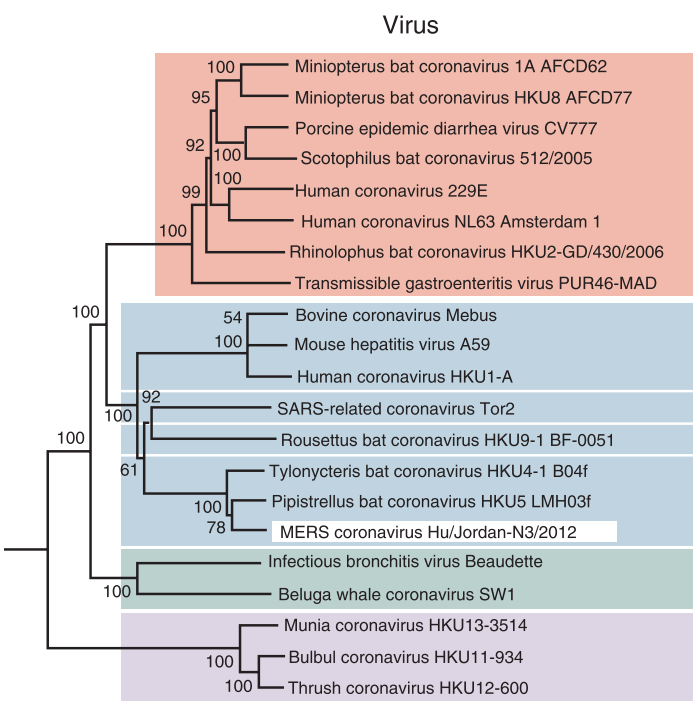
\includegraphics[width=.73\linewidth]{images/38e5046a-099d-4246-ad89-cce1cdf5ea1b-urootedneighborjoiningtree.png}}{}
\makeatother 
\caption{{Rooted neighbor-joining tree}}
\label{f-fcb688b1d4a5}
\end{figure*}
\egroup
It is expected to find similarities between the known human CoVs as all coronavirus genomes share the same baseline structure.\unskip~\cite{689640:16324440} The human CoVs genome is compared using the NCBI-BLAST (National Center for Biotechnology Information Basic Local Alignment Search Tool), results are summarized inTable~\ref{tw-61b03f1ff1e3}. As shown in the table, NL63, OC43, 229E, and MERS share about  $50\% $ of 'identities' and about  $15\% $ of 'gaps' with COVID-19; whereas SARS is the most similar to the novel coronavirus with $80\% $ 'identities' and $1\% $ 'gaps'. 

On the other hand, several media sources have reported the COVID-19 to be from bat provenance. The origin of the novel coronavirus can be confirmed by running a 'Global Alignment' of COVID-19 against the bat coronavirus RaTG13. The alignment reports $96\% $ 'identities' with $0\% $ 'gaps', as shown in Table~\ref{tw-61b03f1ff1e3}. The high percentage of identities and low gaps infers that COVID-19 comes from bats.


\begin{table*}[!htbp]
\caption{{BLAST Global Alignment of the known human CoVs against the novel coronavirus COVID-19} }
\label{tw-61b03f1ff1e3}
\def\arraystretch{1}
\ignorespaces 
\centering 
\begin{tabulary}{\linewidth}{LLLLL}
\tbltoprule Query ID & Virus & NW Score & Identities & Gaps\\
\tblmidrule 
NC\_045512 &
  COVID-19 &
  59806 &
  29903/29903(100\%) &
  0/29903(0\%)\\
NC\_004718 &
  SARS &
  29084 &
  23940/30067(80\%) &
  480/30067(1\%)\\
KF530114 &
  NL63 &
  -11628 &
  17073/31015(55\%) &
  4717/31015(15\%)\\
KX344031 &
  OC43 &
  -10792 &
  18197/32531(56\%) &
  4446/32531(13\%)\\
KF514433 &
  229E &
  -12678 &
  16938/31140(54\%) &
  5212/31140(16\%)\\
KT225476 &
  MERS &
  -8741 &
  18173/31984(57\%) &
  4256/31984(13\%)\\
MN996532 &
  RaTG13 &
  53877 &
  28717/29905(96\%) &
  52/29905(0\%)\\
\tblbottomrule 
\end{tabulary}\par 
\end{table*}
\clearpage 
    

\bibliographystyle{blank}

\bibliography{\jobname}

\section*{Author biography}

\bioItem[images/bf0f1284-fa36-4678-a9e7-05671376e50c-umeitesm]{Antonio Osamu Katagiri Tanaka}{ .

MNT16

A01212611}
\printBio 

\end{document}
